\section{peo\-Agg\-Eval\-Func$<$ EOT $>$ Class Template Reference}
\label{classpeo_agg_eval_func}\index{peoAggEvalFunc@{peoAggEvalFunc}}
The {\bf peo\-Agg\-Eval\-Func}{\rm (p.\,\pageref{classpeo_agg_eval_func})} class offers only the interface for creating aggregate evaluation functions - there are no direct internal functions provided.  


{\tt \#include $<$peo\-Agg\-Eval\-Func.h$>$}

Inheritance diagram for peo\-Agg\-Eval\-Func$<$ EOT $>$::\begin{figure}[H]
\begin{center}
\leavevmode
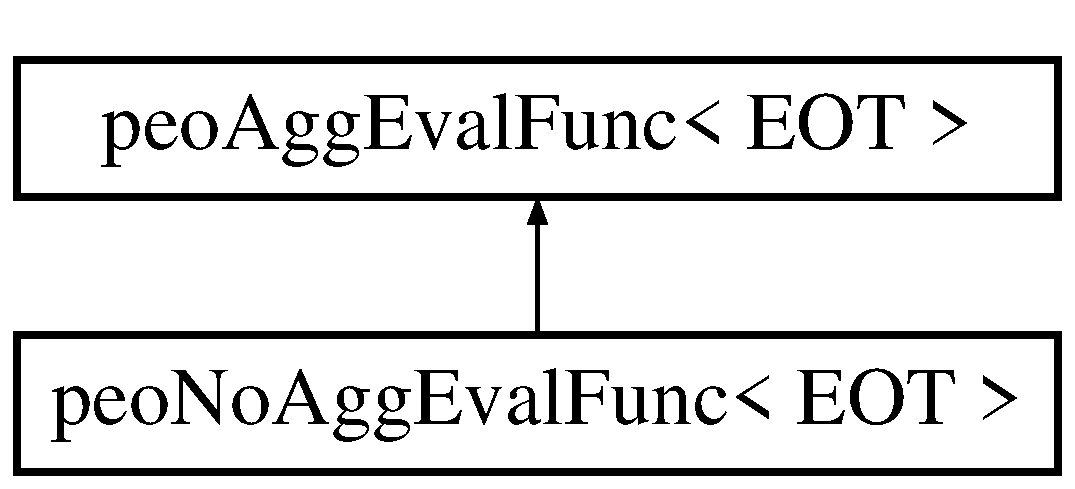
\includegraphics[height=2cm]{classpeo_agg_eval_func}
\end{center}
\end{figure}


\subsection{Detailed Description}
\subsubsection*{template$<$class EOT$>$ class peo\-Agg\-Eval\-Func$<$ EOT $>$}

The {\bf peo\-Agg\-Eval\-Func}{\rm (p.\,\pageref{classpeo_agg_eval_func})} class offers only the interface for creating aggregate evaluation functions - there are no direct internal functions provided. 

The class inherits {\bf public eo\-BF$<$ EOT\&, const typename EOT :: Fitness\&, void $>$} thus requiring, for the derived classes, the creation of a function having the following signature:

\begin{TabularC}{2}
\hline
void operator()( EOT\& \_\-\_\-eot, const typename EOT :: Fitness\& \_\-\_\-partial\_\-fittness ); ~ &~  \\\hline
\end{TabularC}


The aggregation object is called in an iterative manner for each of the results obtained by applying partial evaluation functions. 



Definition at line 40 of file peo\-Agg\-Eval\-Func.h.

The documentation for this class was generated from the following file:\begin{CompactItemize}
\item 
peo\-Agg\-Eval\-Func.h\end{CompactItemize}
